\documentclass[10pt,twocolumn,letterpaper]{article}

\usepackage{cvpr}
\usepackage{times}
\usepackage{epsfig}
\usepackage{graphicx}
\usepackage{amsmath}
\usepackage{amssymb}
\usepackage{multirow}
\usepackage{graphicx}
\usepackage{subfigure}
\usepackage{caption}
\usepackage{bm}

% Include other packages here, before hyperref.

% If you comment hyperref and then uncomment it, you should delete
% egpaper.aux before re-running latex.  (Or just hit 'q' on the first latex
% run, let it finish, and you should be clear).
\usepackage[pagebackref=true,breaklinks=true,letterpaper=true,colorlinks,bookmarks=false]{hyperref}

% \cvprfinalcopy % *** Uncomment this line for the final submission

\def\cvprPaperID{8238} % *** Enter the CVPR Paper ID here
\def\httilde{\mbox{\tt\raisebox{-.5ex}{\symbol{126}}}}

% Pages are numbered in submission mode, and unnumbered in camera-ready
\ifcvprfinal\pagestyle{empty}\fi
\begin{document}

%%%%%%%%% TITLE
\title{Bi-Directional Domain Translation for Zero-Shot Sketch-Based Image Retrieval}

\author{First Author\\
Institution1\\
Institution1 address\\
{\tt\small firstauthor@i1.org}
% For a paper whose authors are all at the same institution,
% omit the following lines up until the closing ``}''.
% Additional authors and addresses can be added with ``\and'',
% just like the second author.
% To save space, use either the email address or home page, not both
\and
Second Author\\
Institution2\\
First line of institution2 address\\
{\tt\small secondauthor@i2.org}
}

\maketitle

\maketitle

\begin{abstract}
   The goal of Sketch-Based Image Retrieval (SBIR) is using free-hand sketches to retrieve images of the same category from a natural image gallery. 
   However, SBIR requires all categories to be seen during training, which cannot be guaranteed in real-world applications. 
   So we investigate more challenging Zero-Shot SBIR (ZS-SBIR), in which test categories do not appear in the training stage. 
   Traditional SBIR methods are prone to be category-based retrieval and cannot generalize well from seen categories to unseen ones. 
   In contrast, we disentangle image features into structure features and appearance features to facilitate structure-based retrieval.
   To assist feature disentanglement and take full advantage of disentangled information, we propose a Bi-directional Domain Translation (BDT) framework for ZS-SBIR, in which the image domain and sketch domain can be translated to each other through disentangled structure and appearance features.
   Finally, we perform retrieval in both structure feature space and image feature space. 
   Extensive experiments demonstrate that our proposed approach remarkably outperforms state-of-the-art approaches by about 8\% on the Sketchy dataset and over 5\% on the TU-Berlin dataset.
\end{abstract}

\section{Introduction}
In recent years, with the rapid growth of multimedia data on the internet, image retrieval is playing a more and more important role in many fields, such as remote sensing and e-commerce. 
Since sketch can be easily drawn and reveal the characteristics of the target images, sketch-based image retrieval (SBIR), which uses a sketch to retrieve the images of the same category, has become widely accepted among users. 
Therefore, SBIR has also attracted widespread attention in research community \cite{del1997visual, cao2010mindfinder, eitz2010evaluation, eitz2010sketch, cao2011edgel, hu2011bag, zhou2012sketch, hu2013performance, cao2013sym, parui2014similarity, james2014reenact, wang2015sketch, saavedra2015sketch, li2016fine, yu2016sketch, qi2016sketch, sangkloy2016sketchy, lu2018learning, saavedra2014sketch}. 
In the conventional setting, it is assumed that the images and sketches in training and test sets share the same set of categories.
However, in real-world applications, the categories of test sketches/images may be out of the scope of training categories.

\begin{figure}
\centering
\includegraphics[width=1\linewidth]{change.pdf}
   \caption{For both seen categories and unseen categories, we visualize the feature of a query sketch (red star) and image features from different categories (points of different colors), which are obtained by SaN \cite{yu2017sketch}, together with the query sketch and an image from the same category.}
\label{fig:inshort}
\vspace{-15pt}
\end{figure}

In this paper, we focus on a more challenging task called zero-shot sketch-based image retrieval (ZS-SBIR) \cite{shen2018zero}, which assumes that test categories do not appear in the training stage. In the remainder of this paper, we refer to training  (\emph{resp.}, test) categories as seen (\emph{resp.}, unseen) categories \cite{dupont2018learning}.
Traditional SBIR methods suffer from sharp performance drop in ZS-SBIR setting \cite{yelamarthi2018zero}, probably because they are prone to learn category-based retrieval.
Specifically, based on the analysis in \cite{yelamarthi2018zero}, since the evaluation methodology is category-based, traditional SBIR methods may take a shortcut by correlating sketches/images with their category labels and retrieving the images from the same category as the query sketch, which is very effective when test data share the same categories as training data. 
However, SBIR methods often fail when the test categories are not present in the training stage. 
As illustrated in Figure~\ref{fig:inshort}, based on the pairwise distance in feature space, SBIR method SaN \cite{yu2017sketch} succeeds in retrieving the images from a seen category ``giraffe" given a query sketch, but fails on an unseen category ``church". We conjecture that to generalize well from seen categories to unseen categories, a model should learn to align the structure information (\emph{e.g.}, outline, shape) of sketches with the corresponding structure information of images (\emph{e.g.}, the structure of church spire in Figure~\ref{fig:inshort}), which is referred to as structure-based retrieval. 

Existing ZS-SBIR methods can be categorized into three groups:
(1) using a generative model based on aligned sketch-image pairs (a sketch is drawn based on a given image and thus has roughly the same outline as this image) to reduce the gap between seen and unseen categories \cite{yelamarthi2018zero}; 
(2) employing semantic information to reduce the intra-class variance in sketches to stabilize the training process \cite{xu2019semantic, wang2019stacked, dutta2019semantically, shen2018zero}; 
(3) fine-tuning the pre-trained model in ZS-SBIR task with semantic-aware knowledge preservation to prevent catastrophic forgetting \cite{liu2019semantic}. 
However, the aligned sketch-image pairs and semantic information are not always available. Moreover, most of the above methods did not achieve the goal of structure-based retrieval. The method in \cite{yelamarthi2018zero} made an attempt at structure-based retrieval but did not explicitly extract structure information from images. 
In terms of the extraction of image structure information, some prior works relied on sketch tokens, which are obtained by extracting the outlines of images \cite{liu2017deep, wang2015sketch, yu2016sketch}. However, the sketch tokens obtained in this way are not very reliable due to the noisy and redundant information, which significantly limits the performance of these methods.

In this work, to facilitate structure-based retrieval, we disentangle image features into structure features and appearance features, where the former encode the structure information (\emph{i.e.}, outline, shape) and the latter encode the additional detailed information (\emph{i.e.}, color, texture).
To assist feature disentanglement and take full advantage of disentangled information, we propose Bi-directional Domain Translation (BDT) framework, where sketches and images are deemed as two domains. 
As shown in Figure \ref{fig:structure}, we first use a pre-trained model to extract features from sketches (\emph{resp.}, images), which are dubbed as sketch (\emph{resp.}, image) features. 
Then, the image features are disentangled into structures features and appearance features, while the sketch features are also projected to the shared structure feature space. 
Furthermore, bi-directional domain translation is performed through the structure features and appearance features.
Concretely, for image-to-sketch translation, we project image features to structure features and then generate sketch features. For sketch-to-image translation, we project sketch features to structure features, which are combined with variational appearance features to compensate the uncertainty when we generate image features from sketch features.
 
Finally, we perform retrieval in both structure feature space and image feature space, to combine the best of two worlds. 
The effectiveness of our proposed BDT framework is verified by comprehensive experimental results on two benchmark datasets. Our main contributions are summarized as follows:
\begin{itemize}
    \item To the best of our knowledge, we are the first to disentangle image features into structure features and appearance features to facilitate structure-based retrieval.
    \item We propose a bi-directional domain translation framework for zero-shot sketch-based image retrieval task.
    \item Comprehensive results on two popular large-scale datasets show that our framework significantly outperforms the state-of-the-art methods.
\end{itemize}

\section{Related Work}

\subsection{SBIR and ZS-SBIR}
The main goal of sketch-based image retrieval (SBIR) is to bridge the gap between image domain and sketch domain. Basically, previous SBIR methods can be categorized into hand-crafted feature based methods and deep learning based methods. Before deep learning was introduced to this task, hand-crafted based methods generally extracted the edge maps from natural images and then matched them with sketches using hand-craft feature \cite{saavedra2015sketch, hu2013performance, eitz2010sketch, hu2011bag, eitz2010evaluation}. In recent years, deep learning based methods have become popular in this area. To reduce the gap between image domain and sketch domain, variants of siamese network \cite{qi2016sketch, sangkloy2016sketchy, song2017deep} and ranking loss \cite{chopra2005learning, sangkloy2016sketchy} were adopted to this task. Besides, semantic information and adversarial loss were also introduced to preserve the domain invariant information \cite{chen2018deep}.

Zero-shot sketch-based image retrieval (ZS-SBIR) was proposed by \cite{shen2018zero} and then followed by \cite{yelamarthi2018zero, xu2019semantic, wang2019stacked, liu2019semantic, dutta2019semantically}. To reduce the intra-class variance in sketches and stabilize the training process, semantic information was leveraged in \cite{wang2019stacked, shen2018zero, xu2019semantic, dutta2019semantically}. To reduce the gap between seen and unseen categories, a generative model along with aligned data pairs, was proposed in \cite{yelamarthi2018zero}. To adapt the pre-trained model to ZS-SBIR without forgetting the knowledge of ImageNet \cite{deng2009imagenet}, semantic-aware knowledge preservation mechanism was used in \cite{liu2019semantic}. However, none of the above methods attempted to disentangle images into structure information and appearance information, which is explored in this work.

\subsection{Disentangled Representation}
Disentangled representation learning aims to divide the latent representation into multiple units, with each unit corresponding to one latent factor (\emph{e.g.}, position, scale, identity). Each unit is only affected by its corresponding latent factor, but not influenced by other latent factors. Disentangled representations are more generalizable and semantically meaningful, and thus useful for a variety of tasks.

Disentangled representation learning methods can be categorized into unsupervised methods and supervised methods according to whether supervision for latent factors is available.
For unsupervised disentanglement, abundant methods have been developed, including InfoGAN \cite{chen2016infogan}, MTAN \cite{liu2018multi}, $\beta$-VAE \cite{higgins2017beta}, JointVAE \cite{dupont2018learning}, FactorVAE \cite{kim2018disentangling}, InfoVAE \cite{zhao2017infovae} and TCVAE \cite{chen2018isolating}. 
Most of them encouraged statistical independence across different dimensions of the latent representation while maintaining the mutual information between input data and latent representations.
For supervised disentanglement, Kingma \textit{et al.}  \cite{kingma2014semi} used disentangled representation to enhance semi-supervised learning. Zheng \textit{et al.} \cite{zheng2019joint} proposed DG-Net to integrate discriminative and generative learning using disentangled representation. Besides, supervised disentanglement has been applied to different tasks, like person re-id \cite{zheng2019joint}, face recognition \cite{liu2018unified, liu2018exploring, shu2017neural, tran2017disentangled}, and image generation \cite{ma2018disentangled, yan2016attribute2image, mathieu2016disentangling, jha2018disentangling}. Our work is the first to apply disentangled representation learning to sketch-based image retrieval task. 

\subsection{Domain Translation}
Many domain translation approaches, like Pix2Pix \cite{pix2pix2017}, CycleGAN \cite{zhu2017unpaired}, BiCycleGAN \cite{zhu2017toward}, StarGAN \cite{StarGAN2018}, DiscoGAN \cite{kim2017learning} have been proposed, which can translate between two domains (\emph{e.g.}, sketch domain and image domain).
In this subsection, we mainly discuss the domain translation methods~\cite{lee2018diverse,lee2019drit,huang2018multimodal,gonzalez2018image} based on disentangled representation. 
Overall speaking, they disentangle latent representation into domain-specific representation and domain-invariant representation. In our problem, structure (\emph{resp.}, appearance) features can be treated as domain-invariant (\emph{resp.}, specific) representation. The translation between two domains in previous works~\cite{lee2018diverse,lee2019drit,huang2018multimodal,gonzalez2018image} is generally symmetric. In contrast, the translation between sketch domain and image domain  is asymmetric because image domain has additional domain-specific representation compared with sketch domain.

\begin{figure*}
\centering
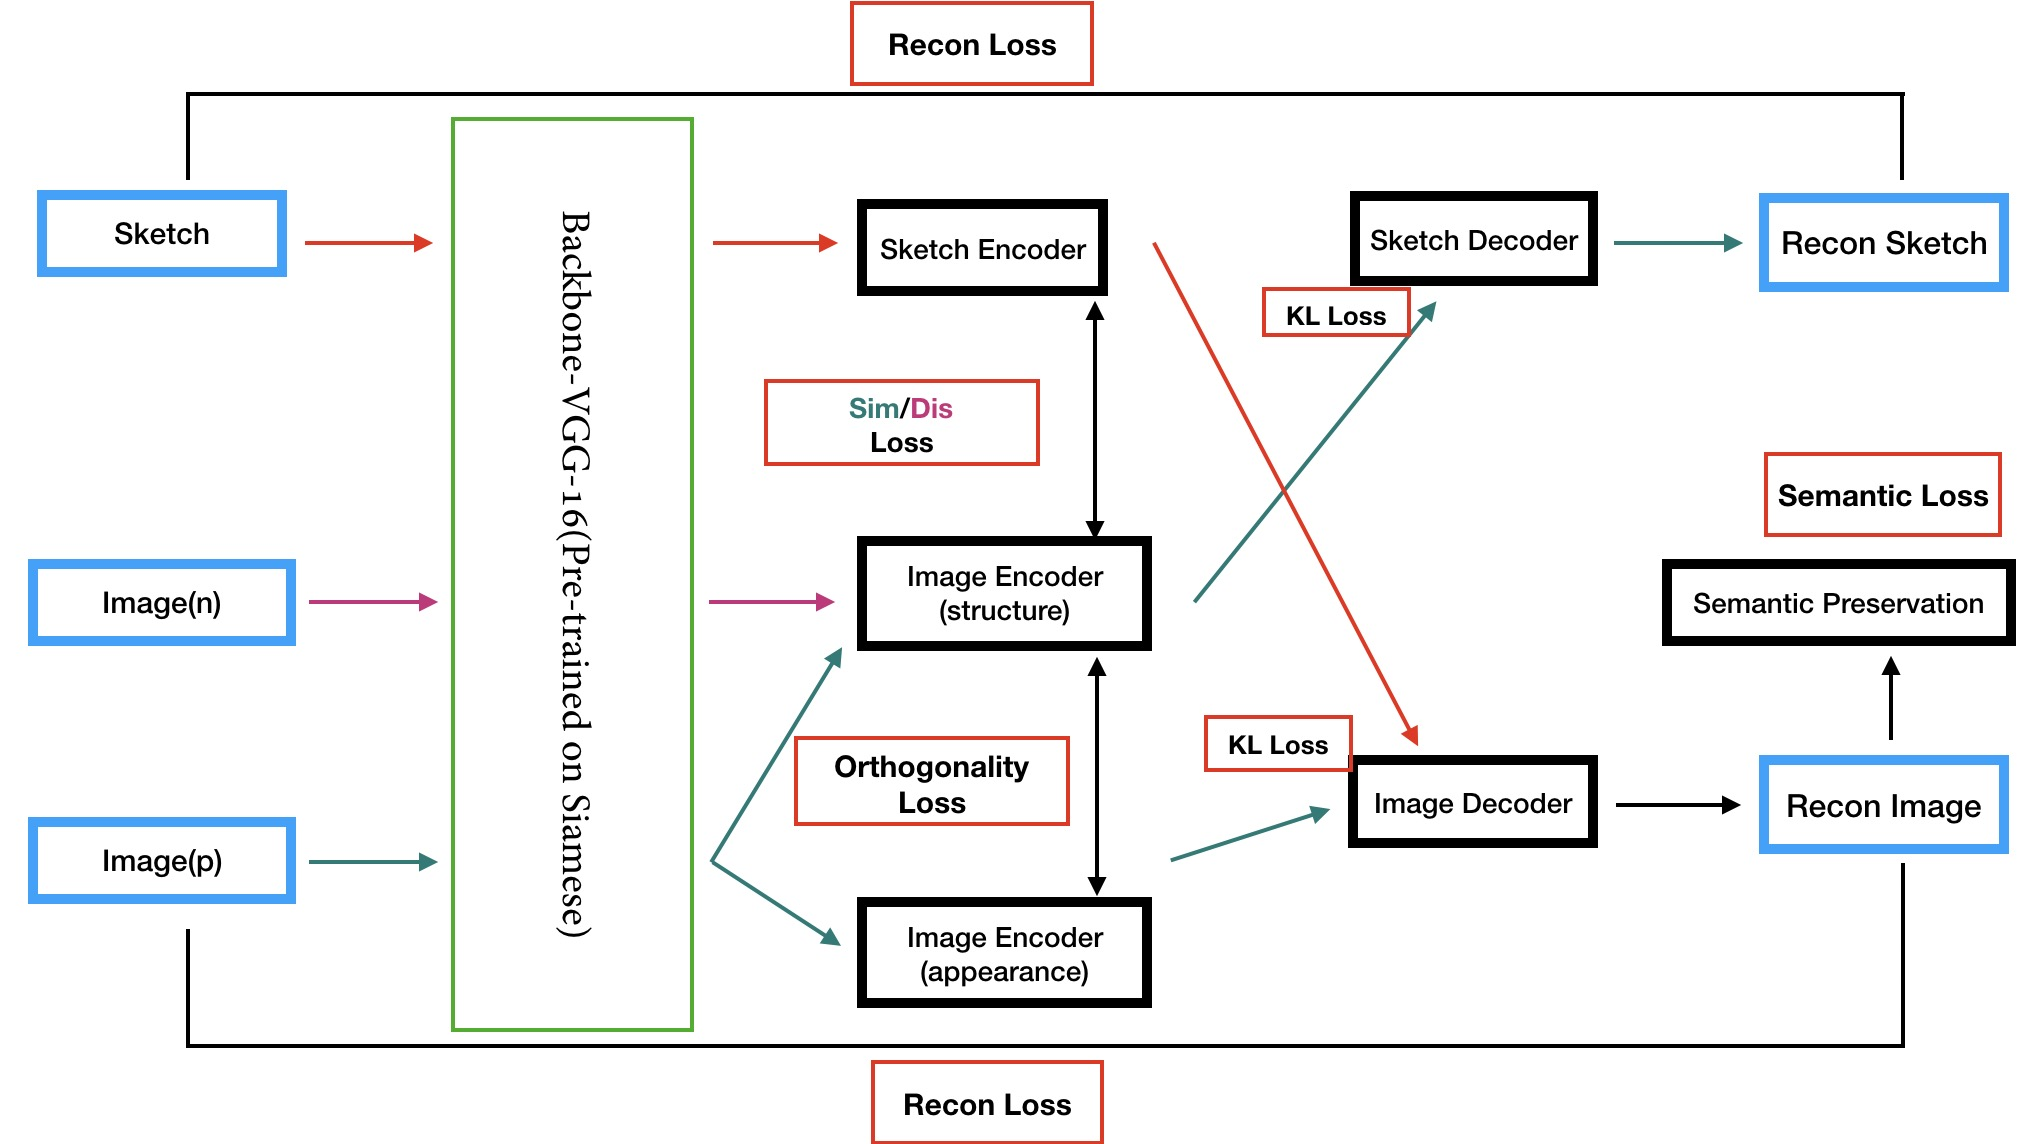
\includegraphics[width=0.95\linewidth]{model_structure.pdf}   
\caption{An overview of our framework. We first adopt VGG-16 \cite{simonyan2014very} to extract features from images and sketch. Then we disentangle image feature into appearance feature and structure feature, through which bi-directional domain translation is performed between image feature space and sketch feature space.}
\label{fig:structure}
\vspace{-10pt}
\end{figure*}

\section{Methodology}
In this section, we introduce our proposed Bi-directional Domain Translation (BDT) framework for zero-shot sketch-based image retrieval. In Sec \ref{3.1}, we state the problem definition. In Sec \ref{3.2}, we elaborate disentangled representation and bi-directional domain translation in detail. In Sec \ref{3.3}, we discuss the strategy during training and retrieval.

\subsection{Problem Definition} \label{3.1}
In this paper, we focus on sketch-based image retrieval under zero-shot setting, where only the sketches and images from seen categories are used in the training stage. 
In the test stage, our proposed framework is expected to use the sketches to retrieve the images, the categories of which are unseen during training.

Formally, we are given a sketch dataset $S_{sk}=\{(\mathbf{x}_i^{sk}, y_i)|y_i \in \mathcal{Y}\}$ and an image dataset $S_{im}=\{(\mathbf{x}_j^{im}, y_j) | y_j \in \mathcal{Y}\}$, where $\mathcal{Y}$ is category label set, and $(\mathbf{x}_i^{sk}, y_i)$ and $(\mathbf{x}_j^{im}, y_j)$ represent the sketches and images with their corresponding category labels respectively.
Following the zero-shot setting in \cite{yelamarthi2018zero,wang2019stacked}, we split all categories $\mathcal{Y}$ into $\mathcal{Y}_{tr}$ and $\mathcal{Y}_{te}$, in which no overlap exists between two label sets, \emph{i.e.}, $\mathcal{Y}_{tr} \cap \mathcal{Y}_{te} = \emptyset$. 
Based on the partition of label set $\mathcal{Y}$, we can split the sketch (\emph{resp.}, image) dataset into $S^{tr}_{sk}$ and $S^{te}_{sk}$ (\emph{resp.}, $S^{tr}_{im}$ and $S^{te}_{im}$).
In the training stage, our model can only process the data in $S^{tr}_{sk}$ and $S_{im}^{tr}$. 
During testing, given a sketch $x_{sk}$ from $S^{te}_{sk}$, our model needs to retrieve the images belonging to the same category as $\mathbf{x}_{sk}$ from test images gallery $S^{te}_{im}$.

The overall framework of our method is illustrated in Figure \ref{fig:structure}. 
We input a triplet containing a pair of sketch $\mathbf{x}_{sk}$ and image $\mathbf{x}_{im}$ from the same category and another image $\mathbf{x}_{im-}$ from a different category. First, a pre-trained model extracts features $\mathbf{f}_{sk}$ (\emph{resp.}, $\mathbf{f}_{im}$ and $\mathbf{f}_{im-}$) from $\mathbf{x}_{sk}$ (\emph{resp.}, $\mathbf{x}_{im}$ and $\mathbf{x}_{im-}$).
Then, image features $\mathbf{f}_{im}$ (\emph{resp.}, $\mathbf{f}_{im-}$) are disentangled into appearance features $\mathbf{f}_{im}^{ap}$ (\emph{resp.}, $\mathbf{f}_{im-}^{ap}$) and structure features $\mathbf{f}_{im}^{st}$ (\emph{resp.}, $\mathbf{f}_{im-}^{st}$). We employ a ranking loss on ($\mathbf{f}_{im-}^{st}$, $\mathbf{f}_{im}^{st}$, $\mathbf{f}_{sk}^{st}$) as well as an orthogonal loss on ($\mathbf{f}_{im}^{st}$, $\mathbf{f}_{im}^{ap}$) to disentangle appearance features and structure features. Furthermore, we use image structure features $\mathbf{f}_{im}^{st}$ to reconstruct sketch features $\mathbf{f}_{sk}$ by using a reconstruction loss and an adversarial loss, because $\mathbf{x}_{sk}$ and $\mathbf{x}_{im}$ belong to the same category. Similarly, we can use sketch structure features $\mathbf{f}_{sk}^{st}$ along with $\mathbf{f}_{im}^{ap}$ to reconstruct $\mathbf{f}_{im}$. To support stochastic sampling in the test stage, we use $\mathbf{f}_{im}^{ap}$ to infer variational appearance features $\mathbf{z}_{im}^{ap}$, which is combined with $\mathbf{f}_{sk}^{st}$ to reconstruct $\mathbf{f}_{im}$. In the test stage, given an image (\emph{resp.}, sketch), we can obtain its structure feature as well as reconstructed (\emph{resp.}, generated) image feature, so that an image and a sketch can be compared in both structure feature space and image feature space. 

\subsection{Our Framework} \label{3.2}

\subsubsection{Feature Extractor} 
Since sketches are highly abstract and visually sparse compared with natural images, it is hard to obtain adequate information from sketches when using a pre-trained model as feature extractor. To tackle this problem without using more parameters, we adopt the fusion strategy in \cite{wang2019stacked} to concatenate the features extracted from multiple layers of the pre-trained model for both images and sketches.

In detail, we first use a pre-trained backbone model, \emph{i.e.}, VGG-16 pre-trained on ImageNet \cite{deng2009imagenet}, to process each sketch and image. 
Suppose $\mathbf{F}_i$ is the output feature of the $i$-th convolution layer and $\mathbf{f}_{fc}$ is the output feature of the last fully connected layer, the final feature $\mathbf{f}$ can be obtained by concatenating $\mathbf{f}_{fc}$ and global average pooling (GAP) of $\mathbf{F}_i$:
\vspace{-10pt}
\begin{align}
\mathbf{f}\!=\![\mathbf{f}_{fc}, GAP(\mathbf{F}_5), GAP(\mathbf{F}_4), GAP(\mathbf{F}_3)].
\end{align}

\subsubsection{Disentangled Representation}
To achieve the goal of structure-based retrieval, we tend to disentangle structure information from image feature. 
Given an image feature $\mathbf{f}_{im}$, we adopt two image encoders $E_{im}^{ap}$ and $E_{im}^{st}$ to disentangle image feature $\mathbf{f}_{im}$ into image structure feature $\mathbf{f}_{im}^{st}$ and image appearance feature $\mathbf{f}_{im}^{ap}$. Besides, to project sketch feature $\mathbf{f}_{sk}$ to the same structure feature space as $\mathbf{f}_{im}^{st}$, a sketch encoder $E_{sk}^{st}$ is adopted to obtain sketch structure feature $\mathbf{f}_{sk}^{st}$. The above process is formulated as follows,
\vspace{-5pt}
\begin{align}
    \mathbf{f}_{im}^{ap} \!=\! E_{im}^{ap}(\mathbf{f}_{im}); \mathbf{f}_{im}^{st} \!=\! E_{im}^{st}(\mathbf{f}_{im}); \mathbf{f}_{sk}^{st} \!=\! E_{sk}^{st}(\mathbf{f}_{sk}).
\end{align}

In each training step, apart from sampling a positive sketch-image pair ($\mathbf{f}_{sk}$, $\mathbf{f}_{im}$) from the same category, we also sample a negative image $\mathbf{f}_{im-}$, which belongs to other categories. Therefore, a triple ($\mathbf{f}_{sk}$, $\mathbf{f}_{im}$, $\mathbf{f}_{im-}$) is fed into the network. We expect that the structure features of images and sketches are in the same feature space. Moreover, in the structure feature space shared by sketch and image, we expect intra-class coherence and inter-class separability across different domains (\emph{i.e.}, sketch domain and image domain). Specifically, we expect to pull sketches close to the images of the same category and push sketches apart from the images of a different category. With the above purpose, we employ a ranking loss with $L_2$ distance:
\vspace{-5pt}
\begin{align} \label{eqn:rank_loss}
        \mathcal{L}_{rk} \!=\! ||\mathbf{f}_{sk}^{st}\!-\!\mathbf{f}_{im}^{st}||_{2}\!+\!\max(0,\!m\!-\!||\mathbf{f}_{sk}^{st}\!-\!\mathbf{f}_{im-}^{st}||_{2}),
\end{align}
in which the margin $m$ is empirically set as 10.0 in our experiments.

After enforcing the structure features of images to share the same structure feature space of sketches, we further expect that the appearance features of images only contain complementary information (\emph{e.g.}, color, texture) to the structure features.
To ensure that the image feature are disentangled in the structure feature space and appearance feature space, we impose an orthogonal constraint on the structure features and appearance features of images based on cosine similarity:
\vspace{-4pt}
\begin{align} \label{eqn:orth_loss}
    \mathcal{L}_{or} = cos(\mathbf{f}_{im}^{ap}, \mathbf{f}_{im}^{sk}) = \frac{\mathbf{f}_{im}^{ap} \cdot \mathbf{f}_{im}^{st}}{||\mathbf{f}_{im}^{ap}||_2 ||\mathbf{f}_{im}^{ap}||_2},
\end{align}
where $\cdot$ means the the dot product between two vectors.
Note that the $\mathbf{f}_{im}^{ap}$ and $\mathbf{f}_{im}^{sk}$ are the output of ReLU activation, so $cos(\cdot}, \cdot)$ is always non-negative and minimizing (\ref{eqn:orth_loss}) will push $cos(\cdot}, \cdot)$ towards zero.

\subsubsection{Bi-directional Domain Translation}
To further help learn disentangled representations and fully utilize the disentangled image features, we perform bi-directional domain translation between sketch domain and image domain.

For image-to-sketch translation, we employ a decoder $G_{sk}$ to reconstruct sketch feature $\mathbf{f}_{sk}$ based on $\mathbf{f}_{im}^{st}$, considering that $\mathbf{f}_{sk}$ and $\mathbf{f}_{im}$ belong to the same category. By denoting $\hat{\mathbf{f}}_{sk} = G_{sk}(\mathbf{f}_{im}^{st})$, we adopt a reconstruction loss $||\mathbf{f}_{sk}-\hat{\mathbf{f}}_{sk}||_2$. Furthermore, we employ an adversarial loss to guarantee that the distribution of generated sketch features is close to that of real sketch features. The adversarial loss is implemented based on a discriminator $D_{sk}$, which distinguishes generated sketch features from real ones. Thus, the total loss of image-to-sketch translation can be written as 
\vspace{-4pt}
\begin{align} \label{eqn:5}
    \mathcal{L}_{tl}^{sk}\!=\!\mathcal{L}_{ad}^{sk}\!+\!\mathcal{L}_{re}^{sk}\!=\!\log(D_{sk}(\hat{\mathbf{f}}_{sk}))\!+\!||\mathbf{f}_{sk}-\hat{\mathbf{f}}_{sk}||_2.
\end{align}

For sketch-to-image translation, we tend to use the sketch structure features to reconstruct image features from the same category. 
However, images contain extra appearance information (\emph{e.g.}, color, texture) compared with sketches, so it is necessary to compensate for the appearance uncertainty when translating from structure features to image features. 
Therefore, image appearance features should be integrated with sketch structure features to reconstruct image features. 

In the test stage, given a sketch, we also hope to generate its imaginary image feature to enable retrieval in the image feature space. Nevertheless, we do not have the corresponding image appearance features in this case. One commonly used solution is stochastic sampling during testing. We introduce a variational estimator $V_{im}^{ap}$ to approximate the variational Gaussian distribution $Q(\mathbf{z}_{im}^{ap}|\mathbf{f}_{im}^{ap})$ based on $\mathbf{f}_{im}^{ap}$ , that is, $(\bm{\mu}_{im}^{ap}, \bm{\sigma}_{im}^{ap})= V_{im}^{ap}(\mathbf{f}_{im}^{ap})$. Then, we use Kullback-Leibler divergence to force  $Q(\mathbf{z}_{im}^{ap}|\mathbf{f}_{im})$ to be close to prior distribution $\mathcal{N}(\mathbf{0}, \mathbf{I})$  with $\mathbf{I}$ being identity matrix to support stochastic sample:
\vspace{-4pt}
\begin{align}
    \mathcal{L}_{KL} = \!-\!D_{KL}(\mathcal{N}(\bm{\mu}_{im}^{ap}, \bm{\sigma}_{im}^{ap}) || \mathcal{N}(\mathbf{0}, \mathbf{I})).
\end{align}

After using reparameterization trick \cite{kingma2013auto} to sample variational appearance feature  $\mathbf{z}_{im}^{ap}$, \emph{i.e.}, $\mathbf{z}_{im}^{ap}=\bm{\mu}_{im}^{ap}+\bm{\epsilon}\circ \bm{\sigma}_{im}^{ap}$, where $\bm{\epsilon}$ is sampled from $\mathcal{N}(\mathbf{0}, \mathbf{I})$ and $\circ$ means element-wise product, we employ a decoder $G_{im}$ to reconstruct $\mathbf{f}_{im}$ based on the concatenation of $\mathbf{z}_{im}^{ap}$ and $\mathbf{f}_{sk}^{st}$.  
By denoting $\hat{\mathbf{f}}_{im} = G_{im}([\mathbf{z}_{im}^{ap}, \mathbf{f}_{sk}^{st}])$, we employ a reconstruction loss $||\mathbf{f}_{im}\!-\!\hat{\mathbf{f}}_{im}||_2$ and an adversarial loss implemented based on the discriminator $D_{im}$, which distinguishes generated image features from real ones, leading to the following loss function:
\vspace{-4pt}
\begin{align} \label{eqn:7}
    \mathcal{L}_{tl}^{im}\!=\!\mathcal{L}_{ad}^{im}\!+\!\mathcal{L}_{re}^{im} \!=\!\log(D_{im}(\hat{\mathbf{f}}_{im})) \!+\! ||\mathbf{f}_{im}\!-\!\hat{\mathbf{f}}_{im}||_2.
\end{align}

By performing image-to-sketch translation, we expect that the image structure features contain the necessary structure information to reconstruct the sketch features from the same category. By performing sketch-to-image translation, we expect that the image appearance features contain the necessary appearance information to compensate for the sketch structure features when reconstructing image features. Therefore, bi-directional domain translation could cooperate with ranking loss and orthogonal loss to assist feature disentanglement.

Finally, recall that the discriminator $D_{im}$ (\emph{resp.}, $D_{sk}$) is trained to distinguish the generated image (\emph{resp.}, sketch) features from the real ones. So the loss functions for discriminators can be written as
\vspace{-4pt}
\begin{align}
    L_{D}^{im} &= \log(1\!-\!D_{im}(\hat{\mathbf{f}}_{im})) \!+\! \log(D_{im}(\mathbf{f}_{im})), \\
    L_{D}^{sk} &= \log(1\!-\!D_{sk}(\hat{\mathbf{f}}_{sk})) \!+\! \log(D_{sk}(\mathbf{f}_{sk})).
\end{align}

\subsection{Training and Retrieval} \label{3.3}

The full objective function can be divided into the generation loss and the discrimination loss, which can be expressed as
\vspace{-5pt}
\begin{align} \label{eqn:total_loss}
    \mathcal{L}_{G} \!&=\! \mathcal{L}_{or} \!+\! \mathcal{L}_{KL} \!+\! \lambda_1 \mathcal{L}_{rk} \!+\!  \lambda_2 \mathcal{L}_{tl}^{im} \!+\! \mathcal{L}_{tl}^{sk}, \\
    \mathcal{L}_{D} &= L_{D}^{im} \!+\!  L_{D}^{sk},
\end{align}
in which $\lambda_1$ and $\lambda_2$ are empirically set as 0.5 and 2.0 respectively. 
Our model consists of generators and discriminators, in order to stabilize the training process, we follow the training strategy in GAN \cite{goodfellow2014generative} to update them alternatingly with $N_{D}$ and $N_{G}$ iterations respectively.

In the test stage, we perform retrieval in both structure feature space and image feature space. Specifically, given a sketch $\mathbf{x}_{sk}$ and an image $\mathbf{x}_{im}$, we compare them in both feature spaces.

1) \textbf{Structure feature space}: We project image feature $\mathbf{f}_{im}$ and sketch feature $\mathbf{f}_{sk}$ into the shared structure feature space by $\mathbf{f}_{im}^{st}=E_{im}^{st}(\mathbf{f}_{im})$ and $\mathbf{f}_{sk}^{st}=E_{sk}^{st}(\mathbf{f}_{sk})$ respectively. Then, we calculate the cosine distance $1\!-\!cos(\mathbf{f}^{st}_{im}, \mathbf{f}^{st}_{sk})$.

2) \textbf{Image feature space}: Based on the sketch structure feature $\mathbf{f}_{sk}^{st}$ and a variational appearance feature sampled from $\mathcal{N}(\mathbf{0},\mathbf{I})$, we can employ the decoder $G_{im}$ to generate an image feature. We can generate $N$ image features vectors by sampling $N$ times ($N=200$ in our experiments) and use the average to represent the final image feature $\hat{\mathbf{f}}_{im}$:
    \vspace{-5pt}
    \begin{align}
        \hat{\mathbf{f}}_{im} = \frac{1}{N}\sum_{i=1}^{N}G_{im}([\mathbf{f}_{sk}^{st}, \mathbf{z}_i]),
    \end{align}
    where $\mathbf{z}_i$ is sampled from $\mathcal{N}(\mathbf{0},\mathbf{I})$. Then, we calculate the cosine distance $1\!-\!cos(\hat{\mathbf{f}}_{im}, \mathbf{f}_{im})$.

Finally, we calculate the weighted average of two distances for retrieval:
\vspace{-5pt}
\begin{equation}
\begin{aligned}
    \mathcal{D}_{fusion} =& \omega (1\!-\!cos(\hat{\mathbf{f}}_{im}, \mathbf{f}_{im})) +  \\
    & (1\!-\!\omega) (1\!-\!cos(\mathbf{f}^{st}_{im}, \mathbf{f}^{st}_{sk})), 
\end{aligned}
\end{equation}
where $\omega$ is a hyper-parameter to balance two feature spaces and set as $0.5$ by default.

\begin{table*}[!htb]
\resizebox{\textwidth}{!}{%
\vspace{-10pt}
\begin{tabular}{cccccccc}
\hline \hline
                         & \multirow{2}{*}{Method} & \multicolumn{2}{c}{Sketchy Ext. (aligned)} & \multicolumn{2}{c}{Sketchy Ext. (unaligned)} & \multicolumn{2}{c}{TU-Berlin Ext.} \\ \cline{3-8} 
                         &                         & P@200(\%)           & mAP@200(\%)          & P@200(\%)            & mAP@200(\%)           & P@200(\%)       & mAP@200(\%)      \\ \hline
\multirow{4}{*}{SBIR}    & Cosine                  & 9.0                   & 5.1                & -                      & -                   & 4.6               & 2.0            \\
                         & 3D shape \cite{wang2015sketch}               & 6.1                   & 1.0                & 7.0                    & 1.8                 & 3.6               & 0.5            \\
                         & SaN \cite{yu2017sketch}                    & 15.3                  & 5.8                & 18.9                   & 8.5                 & 10.1              & 4.2            \\
                         & Siamese \cite{yelamarthi2018zero}                & 24.4                  & 14.6               & 25.6                   & 15.3                & 8.3              & 3.7            \\ \hline
\multirow{5}{*}{ZSL}     & ESZSL \cite{romera2015embarrassingly}                  & 16.0                  & 8.3               & 17.2                   & 9.5                & 4.8               & 1.7            \\
                         & SAE  \cite{kodirov2017semantic}                   & 24.4                  & 14.6               & 27.1                   & 17.5                & 11.6              & 5.5            \\
                         & CMT \cite{socher2013zero}                    & 26.9                   & 17.6                & 27.5                    & 17.7                 & 10.0               & 4.3            \\
                         & SSE \cite{zhang2015bit}                    & 6.9                   & 2.3                & 7.3                    & 3.3                 & 4.1               & 1.2            \\
                         & DeViSE \cite{frome2013devise}                 & 14.3                   & 4.7                & 15.4                    & 5.4                 & 8.0               & 2.2            \\ \hline
\multirow{6}{*}{ZS-SBIR} & CVAE \cite{yelamarthi2018zero}                   & 33.4                  & 22.6               & 31.2                   & 19.9                & 10.2              & 4.9            \\
                         & SEM-PCYC \cite{dupont2018learning}                   & 28.0                  & 17.7               & 30.0                   & 19.4                & 12.4              & 5.7            \\
                         & Xu \textit{et al.} \cite{xu2019semantic}         & 20.4                  & 12.0               & 20.8                        & 12.6                & 7.4               & 2.9                \\
                         & \textbf{BDT-St}            & 36.1                  & 25.5               & 36.9                   & 25.8                & 15.2              & 7.9           \\
                         & \textbf{BDT-Im}            & 37.2                  & 26.8               & 35.1                   & 24.9                & 14.7              & 7.1           \\
                         & \textbf{BDT}            & \textbf{41.2}            & \textbf{29.9}      & \textbf{39.7}          & \textbf{28.1}       & \textbf{17.6}              & \textbf{10.2}           \\ \hline \hline
\end{tabular}%
}
\vspace{-6pt}
\caption{Comparison of our BDT method and baselines on Sketchy and TU-Berlin. Best results are denoted in boldface.}
\label{tab:1}
\vspace{-15pt}
\end{table*}

\section{Experiment}

\subsection{Experiment Setup}

\subsubsection{Dataset}
We evaluate our BDT framework and baselines on two large-scale sketch-image datasets: TU-Berlin \cite{eitz2012hdhso} and Sketchy \cite{sangkloy2016sketchy} with extended images obtained from \cite{liu2017deep}.

\textbf{Sketchy} (Extended) \cite{sangkloy2016sketchy} is originally comprised of 75,479 sketches and 12,500 images from 125 categories, where the images and sketches are aligned pairs. Liu \textit{et al.} \cite{liu2017deep} extended the image retrieval gallery by collecting extra 60,502 images, so that the total number of images in extended Sketchy reaches 73,002. Following the standard zero-shot setting in \cite{yelamarthi2018zero}, we partition the total 125 categories into 104 seen categories and 21 unseen categories according to whether the category appears in the 1,000 categories of ImageNet-1k \cite{deng2009imagenet}, which avoids violating the zero-shot assumption when utilizing models pre-trained on ImageNet-1k. In the training stage, there were previously two settings about how to utilize the training data: 1) use aligned pairs without extended training images \cite{yelamarthi2018zero}, which is referred to ``aligned" in Table~\ref{tab:1}; 2) do not use the information of aligned pairs but use all training data including extended images \cite{shen2018zero}, which is referred to as ``unaligned" in Table~\ref{tab:1}.

\textbf{TU-Berlin} (Extended) \cite{eitz2012hdhso} contains 250 categories with a total of 20, 000 sketches extended by \cite{liu2017deep} with 204,489 natural images from the sketch categories. Following the same split criterion as Sketchy, we first split the TU-Berlin into 165 seen categories and 85 unseen categories according to whether the category appears in the 1,000 categories of ImageNet-1k \cite{deng2009imagenet}. As Shen \textit{et al.} \cite{shen2018zero} suggested, we re-select unseen categories with more than 400 images out of the 85 categories. In the end, there are 186 seen and 64 unseen categories. Compared with the Sketchy dataset, TU-Berlin is much more challenging because of more unseen categories and fewer training sketches.

\subsubsection{Implementation Details}
We implement our method and all the other baselines using PyTorch \cite{paszke2017automatic}, which are all trained on one GTX 1080Ti GPU. We use a VGG-16 (pre-trained on ImageNet dataset) to extract the image and sketch features. As Sec. \ref{3.2} mentioned, we concatenate the output of multiple layers, leading to a 5568-dim vector for each image and sketch. For each encoder, we use two fully-connected (FC) layers with Batch Normalization and ReLU as activation. For the variational estimator, we use two individual FC layers to obtain the mean and variance of approximated $\mathbf{z}_{im}^{ap}$ separately. For each decoder, we use two FC layers with ReLU activation. For discriminators, we use two FC layers with Batch Normalization and LeakyReLU as activation. The dimensionality of $\mathbf{f}_{sk}^{st}$, $\mathbf{f}_{im}^{st}$, $\mathbf{f}_{im}^{ap}$, $\mathbf{z}_{im}^{ap}$ are all 1024.

We use Adam \cite{kingma2014adam} optimizer with learning rate $2 \times 10^{-4}$, $\beta_1 = 0.5$, $\beta_2 = 0.999$ for bi-directional translation model, and use SGD optimizer with learning rate $1 \times 10^{-2}$, momentum $=0.9$ for the discriminators. The batch size for Sketchy (\emph{resp.}, TU-Berlin) is 128 (\emph{resp.}, 64) and the maximum number of training epochs is 30. The numbers of iterations for training generator ($N_{G}$) and discriminator ($N_{D}$) are 100 and 50 respectively. For Sketchy dataset, we conduct experiments in both ``unaligned" and ``aligned" settings (see Table~\ref{tab:1}), whereas there is only ``unaligned" setting for TU-Berlin dataset because TU-Berlin does not have aligned pairs. Following \cite{yelamarthi2018zero}, we use mean average precision and precision considering top 200 retrievals (mAP@200 and P@200) as the evaluation metric.

\subsection{Comparison with Existing Methods}
We compare our model with $12$ prior methods, which can be divided into three categories: sketch-based image retrieval (SBIR) baselines, zero-shot learning (ZSL) baselines, zero-shot sketch-based image retrieval (ZS-SBIR) baselines. 
The SBIR baselines include Siamese \cite{yelamarthi2018zero}, SaN \cite{yu2017sketch}, and 3D shape \cite{wang2015sketch}. A cosine baseline is also added, which conducts nearest neighbor search based on 4096-dim VGG-16 \cite{simonyan2014very} feature vectors.
The ZSL baselines include ESZSL \cite{romera2015embarrassingly}, SAE \cite{kodirov2017semantic}, CMT \cite{socher2013zero}, SSE \cite{zhang2015bit}, and DeViSE \cite{frome2013devise}.
The ZS-SBIR baselies include CVAE \cite{yelamarthi2018zero}, SEM-PCYC \cite{dutta2019semantically}, and Xu \textit{et al.} \cite{xu2019semantic}.
For a fair comparison, we replace the backbone of all previous models by VGG-16 except SaN, which designs a new backbone to extract sketch and image features. 
All the backbones are pre-trained on ImageNet. 
Note that our method does not rely on semantic information obtained from large textual corpus (\emph{e.g.}, word vector \cite{mikolov2013distributed} and WordNet \cite{miller1998wordnet}). To make a fair comparison, for those baselines which require additional semantic information, we remove the semantic information \cite{dutta2019semantically} or replace the semantic information by the average of image features within each category \cite{wang2015sketch, romera2015embarrassingly, kodirov2017semantic, socher2013zero, zhang2015bit, frome2013devise, xu2019semantic} \protect\footnotemark[1]. In fact, we have tried both ``remove" and ``replace" strategies for each baseline, and select the better one for each baseline.
Besides, we do not compare with the methods that fine-tune the pre-trained backbone during training, like SAKE \cite{liu2019semantic} and EMS \cite{lu2018learning}, because they learn four times more model parameters than ours.

\footnotetext[1]{The results of ZSIH \cite{shen2018zero} become much worse after using this strategy, and thus we omit its results in Table~\ref{tab:1}.}

\begin{table}[]
\setlength{\tabcolsep}{0.3mm}{
\resizebox{0.50\textwidth}{!}{
\begin{tabular}{lcccc}
\hline \hline
 & \multicolumn{2}{c}{Sketchy Ext. (aligned)} & \multicolumn{2}{c}{Sketchy Ext. (unaligned)} \\ \cline{2-5} 
\multicolumn{1}{c}{} & P@200(\%) & mAP@200(\%) & P@200(\%) & mAP@200(\%) \\ \hline
w/o $L_{rk}$ & 35.1 & 23.2 & 31.7 & 20.3 \\
w/o $L_{or}$ & 40.3 & 29.1 & 38.4 & 26.9 \\
w/o $L_{re}^{im}$ & 31.7 & 19.8 & 32.1 & 20.5 \\
w/o $L_{re}^{sk}$ & 39.9 & 28.3 & 38.3 & 27.8 \\
w/o $L_{ad}^{im}$ & 40.0 & 28.3 & 35.5 & 24.9 \\
w/o $L_{ad}^{sk}$ & 40.7 & 29.6 & 39.3 & 27.9 \\
alternative $L_{or}$ & 39.1 & 27.4 & 37.9 & 26.6 \\
w/o appearance & 37.2 & 26.0 & 36.5 & 25.9 \\ \hline \hline
\end{tabular}
}}
\caption{Ablation Studies of our method on Sketchy dataset.}
\label{tab:2}
\vspace{-15pt}
\end{table}


Based on Table~\ref{tab:1}, we can find that most of the SBIR and ZSL baselines under-perform the ZS-SBIR baselines. 
Compared with Cosine, 3D shape \cite{wang2015sketch} and DeViSE \cite{frome2013devise} perform ever worse, which indicates these methods heavily overfit on the seen categories. 
On Sketchy dataset, we observe that the results in ``unaligned" setting are usually better than the corresponding results in ``aligned" setting, mainly because that the amount of unaligned data is five times larger than that of aligned data.
However, CVAE exhibits the opposite tendency because the aligned sketch-image pairs could help reconstruct images from their paired sketches. 
On the TU-Berlin dataset, the overall results are worse than those reported in previous works \cite{liu2019semantic, dutta2019semantically} due to different seen/unseen splits. 
In particular, the number of unseen categories under our split is two times larger than that in  \cite{liu2019semantic, dutta2019semantically}, and our split criterion also guarantees no information leak from ImageNet to unseen categories.

In terms of P@200, our proposed BDT excels the state-of-the-art methods by 7.8\% on the Sketchy (aligned) dataset, 8.5\% on Sketchy (unaligned) dataset, and 5.2\% on TU-Berlin dataset. 
To better understand our method, we also list our results by performing retrieval only in the image feature space or structure space as \textbf{BDT-Im} and \textbf{BDT-St}, respectively. Referring to the comparison between \textbf{BDT-Im} and CVAE as well as the comparison between \textbf{BDT-St} and Siamese, the disentangled representations indeed help the model to generalize from seen to unseen categories. 
Besides, by comparing \textbf{BDT} with \textbf{BDT-Im} and \textbf{BDT-St}, we can see that the combination of image feature space and structure feature space can boost the performance by a large margin, which indicates the complementarity of two feature spaces.

\begin{figure}
\begin{center}
\includegraphics[width=1\linewidth]{combine.pdf}
\end{center}
\vspace{-15pt}
   \caption{a. The performance variance of our method when setting $\omega$ in the range of $[0, 1]$, where Sk (a), Sk(u) and TU represent Sketchy (aligned), Sketch (unaligned) and TU-Berlin respectively. b. The performance and orthogonality variance of our method along with the training epoch.}
\label{fig:orth}
\vspace{-15pt}
\end{figure}

\begin{figure*}
\begin{center}
\includegraphics[width=1\linewidth]{casestudy2.pdf}
\end{center}
\vspace{-10pt}
   \caption{The top-5 images retrieved by BDT, BDT-St, BDT-Im, CVAE methods on Sketchy (Aligned) dataset. The green (\emph{resp.}, red) border indicates the correct (\emph{resp.}, incorrect) retrieval results.}
\label{fig:case}
\vspace{-14pt}
\end{figure*}

\subsection{Ablation Study}
By taking the Sketchy dataset as an example, we analyze the effect of different loss functions and alternative model designs as well as the effect of $\omega$.

\noindent\textbf{Study on loss terms: }
We ablate each loss term in (\ref{eqn:rank_loss}), (\ref{eqn:orth_loss}), (\ref{eqn:5}) and (\ref{eqn:7}), and report the results in Table \ref{tab:2}. As expected, the ranking loss and the image reconstruction loss are the most important losses, because these two losses mainly control the image-sketch distance in their corresponding feature spaces. Besides, the image reconstruction loss has larger impact in ``aligned" setting than ``unaligned" setting, which implies that the reconstruction loss is sensitive to the pose variance in unaligned data. In contrast, the image adversarial loss has larger impact in ``unaligned" setting, which shows that the adversarial loss can enhance the robustness of our model in ``unaligned" setting.

\noindent\textbf{Study on alternative model designs: }
In the last two rows in Table \ref{tab:2}, we report the results of two alternative designs: (1) move the orthogonal loss from ($\mathbf{f}_{im}^{ap}, \mathbf{f}_{im}^{st}$) to ($\mathbf{z}_{im}^{ap},\mathbf{f}_{im}^{st}$); (2) directly translate from sketch structure feature to image feature without using the image appearance feature $\mathbf{z}_{im}^{ap}$. We can observe the performance drop in both cases, which demonstrates that we have placed the orthogonal loss at the proper position, and the appearance compensation is crucial for generating image features.

\noindent\textbf{Study on retrieval strategy: }
In Figure \ref{fig:orth}\color{red}a\color{black}, we plot the $\omega$-P@200 curve. It can be seen that our method can generally achieve competitive results when setting $\omega$ in a proper range, \emph{e.g.}, $[0.4, 0.6]$. 

\subsection{Disentanglement Analysis}
To demonstrate the ability of our model to disentangle the image features, we first plot orthogonal loss and P@200 along with the training epoch in Figure \ref{fig:orth}\color{red}b\color{black}. It can be seen that the orthogonal loss decreases as P@200 increases, which indicates that our method benefits from the disentanglement of image features.

\begin{figure}
\begin{center}
\includegraphics[width=1\linewidth]{tsne.pdf}
\end{center}
\vspace{-10pt}
   \caption{The t-SNE visualization of six types of features on Sketchy test set. Best viewed in color.}
\label{fig:tsne}
\vspace{-15pt}
\end{figure}

Then, in Figure \ref{fig:tsne}, we visualize six types of features from 10 randomly selected unseen categories using t-SNE \cite{maaten2008visualizing}: image appearance features, image structure features, sketch features, sketch structure features, sketch translated image features. According to Figure \ref{fig:tsne}, we have the following observations: 1) Different categories can be separated very well in ``image structure" and ``sketch structure", which significantly facilitates the retrieval in structure feature space; 2) The results in ``image structure" and ``image appearance" are complementary, in accordance with the disentanglement between structure features and appearance features; 3) The results in ``image features" and ``translated image features" are similar, which shows the effectiveness of image feature reconstruction; 4) The results in ``sketch feature" show the relatively poor separability of sketch features, which makes sketch feature space ill-suited for image retrieval.

\subsection{Case Study}
In Figure \ref{fig:case}, we show the retrieval results of \textbf{BDT-St}, \textbf{BDT-Im}, \textbf{BDT}, and CVAE \cite{yelamarthi2018zero}. One interesting observation is that BDT-ST could capture the correspondence of local structure information, while BDT-Im behaves like CVAE and focuses on global pose/structure information. For example, given a ``door" sketch, the retrieved images of both CVAE and BDT-Im have the global grid structure similar to the given sketch, but BDT-St could capture the correspondence between the retrieved images and the given sketch \emph{w.r.t.} certain local structure information like door-case.
One possible explanation is that the structure features are trained by aligning different domains into a shared space; however, the reconstructed image features are trained by aligning the sketch features to image features, which makes the former one more flexible and tolerant to the difference between image and sketch. 
Moreover, BDT combines the strengths of both BDT-St and BDT-Im, producing better retrieval results.


\section{Conclusion}
We have studied zero-shot sketch-based image retrieval (ZS-SBIR) from a new viewpoint, \emph{i.e.}, using disentangled representation to facilitate structure-based retrieval. We have proposed our Bi-directional Domain Translation (BDT) framework, which performs retrieval in two feature spaces. Comprehensive experiments on Sketchy (aligned/unaligned) and TU-Berlin datasets have demonstrated the generalization ability of our framework from seen categories to unseen categories.

{\small
\bibliographystyle{ieee_fullname}
\bibliography{egbib}
}

\end{document}
